\subsection*{Progress beyond state of the art}

\begin{longtable*}{|p{0.2\textwidth}|p{0.75\textwidth}|}
\hline
{\bf Networking activities}
&
In order to foster a culture of cooperation between scientific
communities that are often too focused on their own problems, this project
will develop several types of networking activities.\\
&
\hspace{0.4cm}
The initial phase of the project, the development of a common
infrastructure, will be the first step in the networking activities of
the twenty-eight project partners. Thereafter, collaborations between
partners will grow, allowing them to better use the Logipedia
infrastructure to meet their needs as well as those of users outside
the project. This effort will develop the formal proof community in
the countries where it is still in an early stage of development.  To
structure this growth, several user groups will be created: 
in industry, in academia, in education, and in publishing.\\
&
\hspace{0.4cm}
The industrial partners of the project
and the {\bf club of industrial users} 
will strengthen a culture of cooperation between scientific
researchers and engineers in academia and in industry. Currently, this
cooperation is too often point-to-point (for instance, an enterprise uses
one system and develops links to a group of academic researchers
developing this system). But we need to develop a more comprehensive
culture of cooperation, around common languages and a common research
infrastructure.\\
&
\hspace{0.4cm} Our action in this direction is twofold. First, some
enterprises that already have a strong commitment in formal methods
(Clearsy, CEA, Runtime Verification, etc.) are included in the project as
partners. Other enterprises that could not be part of the project
because of its limited size, or that have a less developed culture in
formal methods, are members of the club of industrial users. Among
other goals, this club participates to develop a culture of
technology watch in formal methods in industry, which is a stepping
stone for developing a strong industrial awareness in safety and
security in European industry. This club is also only in its initial
phases, but we are confident that the initial members of this club
will be followed by others.\\ 
&
\hspace{0.4cm}
The {\bf club of academic users}
will develop a similar culture of technology watch for
researchers who are outside formal methods.  
It gathers colleagues from our community that could not participate to
this project, as well as colleagues from outside the formal methods
community, in particular mathematicians who are understanding
the long term impact formal proofs will have on mathematics.\\
&
\hspace{0.4cm}
The {\bf club of users in education}
will also to develop a similar culture of
technology watch for teachers, including high school teachers who are
investigating how a library of formal proofs can be used with younger
students. Here we do not advocate teaching formal proofs to pre-schoolers, but
we aim at fostering a culture of rigour in high-school mathematical
thinking, by having rigorous statements of theorems in high-school
textbooks (including all the corner cases that are often omitted), as
well as a clear structure of how each proof of a theorem relies on
other theorems. This improved rigour is useful for both the students
who will study sciences at University and to those who will not. In
particular, in this way we want to modestly contribute to the renewal
of the logical thinking culture, which is of prime importance in our
``post-truth era''.\\
&
\hspace{0.4cm}
We also believe that an early exposition to formal statements and / or
formal proofs may contribute to compensate the gender disparity
in our research community. Here also, we must remain modest, as
achieving a decent gender-balance will require more than a single
action, but is obviously much more effective to try to promote
contemporary scientific ideas, and encourage scientific carriers, to
women at the high school level rather that at the university level,
because at the university level there are already too few women in
our auditoriums.\\
&
\hspace{0.4cm}
The more inceptive {\bf club of users in publishing} 
will develop networking activities with publishers
(Elsevier, Springer, etc. but also, ArXiv, HAL, Wikipedia, etc.)~
such that formal proofs mentioned in research papers and in
other encyclopedia can be permanently made accessible, in Logipedia, 
while they currently often are just made accessible
on the web page of the authors.\\
&
\hspace{0.4cm}
These four clubs of users: industrial users, academic users, users in 
education, and users in publishing, together with the partners of the 
project, will also
prepare a larger community that will develop Logipedia beyond the end
of the project, in order to achieve our ultimate goal of making
Logipedia contain all the formal proofs then developed in twenty
years.\\
%% &
%% \begin{center}
%% 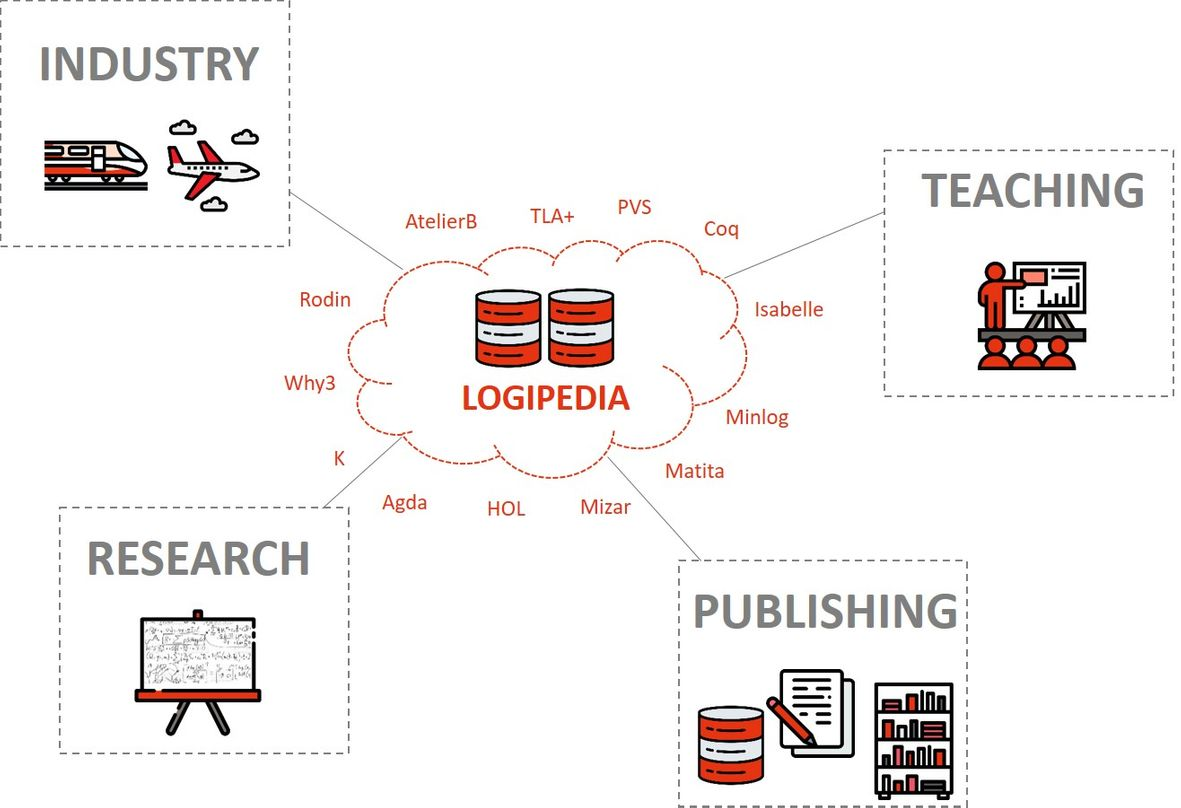
\includegraphics[width=12cm]{img/Schema-reduced}
%% \end{center}\\
&
\hspace{0.4cm}
Finally, this project also prepares the exploitation of Logipedia
beyond the duration of the project.\\
&
\hspace{0.4cm}
Of course, we also plan to organise other networking activities,
such as a yearly conference with associated workshops on applications
in industry, research, education, and publishing, a general assembly
where the research directions can be discussed collectively. We also plan to organise
summer schools, especially at the beginning of the project in order to
train the new participants (doctoral students, post-docs, etc.) to the
technology developed in Dedukti and Logipedia
(see Section Dissemination and Communication.)\\
&
\hspace{0.4cm}
So developing jointly such an infrastructure will not only reconfigure
the research community on formal methods, but also the industrial
community on formal methods, and will build bridges with the communities
of education and of publishing.\\
\hline
{\bf Trans-national access and virtual access}
&
Logipedia will be accessible online. It will therefore be accessible
at no cost, and without identification, from every country in Europe
and beyond, just like, for instance, Wikipedia is.\\
&
\hspace{0.4cm} The licence chosen for the Logipedia proofs does not
need to be the same for all proofs, because some proofs already have a
licence before being imported in Logipedia and, in some cases, this
licence must be preserved.  Yet, in general we will favour a Creative
Commons licence and, in particular, cc-by.  Such a licence allows a free
access, a findable, accessible, interoperable, and reusable data
management. It will contribute to the development of the Open data /
Open science / Open innovation philosophy and be in line with European
policies encouraging open science.
\\
&
\hspace{0.4cm} Being a central infrastructure, Logipedia will
contribute to strengthen the links within the European research area,
that it too scattered: for instance, currently, researchers and
engineers often use a system developed in their own country (only a
few systems having an international community of users), and the
libraries of formal proofs specific to this system.
\\
&
\hspace{0.4cm}
As explained above, our effort on access goes beyond providing a
trans-national and virtual access, as accessibility depends also on
developing an ergonomic web interface, a package distribution system,
a search engine, and an ontology of mathematical concepts. The public
targeted by these interfaces also has to be taken into account, a
secondary school student looking for a theorem in geometry needs a
different interface from a engineer looking for the correctness proof
of an algorithm.\\
\hline
{\bf Joint research activities}
&
The project includes joint research activities that would not be possible 
without this project of co-building an infrastructure.
\\
&
\hspace{0.4cm} Logipedia will allow joint research projects between
the users of this infrastructure that will be able to develop new
proofs together using different systems.\\
&
\hspace{0.4cm}
Then, Logipedia raises new research
problems. Some of them have already been solved in the past and
must be implemented jointly. Others are newer.\\
&
\hspace{0.4cm}
Using a common infrastructure requires
to describe the theories implemented in the different systems in a
common logical framework. We have already discussed how the expression
of geometry, arithmetic, and set theory in predicate logic has
enabled a renewal of logic at the end of the 1920's, allowing all
the logicians to speak the same language. Here we can expect a similar
renewal, fostering new joint research through the sharing, not
only of a common infrastructure, but also of a common language.\\
&
\hspace{0.4cm}
The development of a common encyclopedia, such as Logipedia, also
raises completely new problems such as automatic concept alignment,
structuring a large body of knowledge, or the development of
interfaces. These problems will trigger new cooperation between the
partners of the project and beyond.\\
\hline
\end{longtable*}


%%% Local Variables:
%%%   mode: latex
%%%   mode: flyspell
%%%   ispell-local-dictionary: "british"
%%% End:
